\documentclass{article}

\usepackage[english]{babel}
\usepackage[utf8]{inputenc}
\usepackage{amsmath,amssymb}
\usepackage{parskip}
\usepackage{graphicx}
\usepackage{listings}
\usepackage{float}
\usepackage{subfig}

\lstset{
    numbers=left, 
    numberstyle= \tiny, 
    keywordstyle= \color{ blue!70},
    commentstyle= \color{red!50!green!50!blue!50}, 
    frame=shadowbox, % 阴影效果
    rulesepcolor= \color{ red!20!green!20!blue!20} ,
    escapeinside=``, % 英文分号中可写入中文
    xleftmargin=2em,xrightmargin=2em, aboveskip=1em,
    framexleftmargin=2em,
    breaklines=true,
    language=c++
} 
% Margins
\usepackage[top=2.5cm, left=3cm, right=3cm, bottom=4.0cm]{geometry}
% Colour table cells
\usepackage[table]{xcolor}

% Get larger line spacing in table
\newcommand{\tablespace}{\\[1.25mm]}
\newcommand\Tstrut{\rule{0pt}{2.6ex}}         % = `top' strut
\newcommand\tstrut{\rule{0pt}{2.0ex}}         % = `top' strut
\newcommand\Bstrut{\rule[-0.9ex]{0pt}{0pt}}   % = `bottom' strut

%%%%%%%%%%%%%%%%%
%     Title     %
%%%%%%%%%%%%%%%%%
\title{CSCI803 Assignment}
\author{Yao Xiao \\ SID 2019180015}
\date{\today}

\begin{document}
\maketitle

%%%%%%%%%%%%%%%%%
%   Problem 1   %
%%%%%%%%%%%%%%%%%
\section{Task 1}
\begin{lstlisting}
public class Fibonacci{
	public static int fibDP(int x) {
			int fib[] = new int[x + 1];
			fib[0] = 0;
			fib[1] = 1;
			for (int i = 2; i < x + 1; i++) {
				fib[i] = fib[i - 1] + fib[i - 2];
			}
		return fib[x];
		}
	public static int main(String[] args){
        System.out.println(fibDP(10));
        return 0;
	}
}    
\end{lstlisting}


\section{Task 2}
\begin{lstlisting}
#include <iostream>
#include <stdio.h>
#include <time.h>
#include "/usr/local/Cellar/libomp/11.0.0/include/omp.h"

using namespace std;

void merge_sort_recursive(int arr[], int reg[], int start, int end) {
    if (start >= end)
        return;
    int len = end - start, mid = (len >> 1) + start;
    int start1 = start, end1 = mid;
    int start2 = mid + 1, end2 = end;
    omp_set_num_threads(12);
#pragma omp task
    merge_sort_recursive(arr, reg, start1, end1);
#pragma omp task
    merge_sort_recursive(arr, reg, start2, end2);
    int k = start;
    while (start1 <= end1 && start2 <= end2)
        reg[k++] = arr[start1] < arr[start2] ? arr[start1++] : arr[start2++];
    while (start1 <= end1)
        reg[k++] = arr[start1++];
    while (start2 <= end2)
        reg[k++] = arr[start2++];
    for (k = start; k <= end; k++)
        arr[k] = reg[k];
}

int *merge_sort(int arr[], int len) {
    int reg[100000];
    merge_sort_recursive(arr, reg, 0, len - 1);
    return arr;
}

int main() {
    int arr[100000];
    int num_start = 1;
    int num_end = 100001;
    double duration;
    clock_t start, end;
    printf("Generating random numbers...\n");
    for (int i = 0; i < 100000; ++i)
        arr[i] = (rand() % (num_end - num_start)) + num_start;
    start = clock();
#pragma omp parallel
    {
#pragma omp single nowait 
        merge_sort(arr, 100000);
    }
    end = clock();
    duration = (double) (end - start);
    printf("Time Using is:%f\n", (duration / CLOCKS_PER_SEC));
    return 0;
}

\end{lstlisting}

\subsection{Comparsion}
\begin{figure}[H]
    \subfloat[][Single thread computing without OpenMP]{
        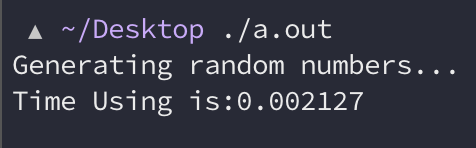
\includegraphics[width=1\textwidth]{Fig2}}\\
    \subfloat[][Multithread parallel computing using OpenMP]{
        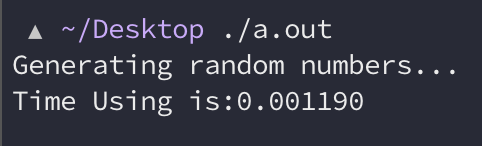
\includegraphics[width=1\textwidth]{Fig1}}
\end{figure}

Since my CPU has 6 cores and 12 threads, it can be seen from the figure above that CPU power consumption is the largest, the computing speed is the fastest, and the consumption time is the smallest.
\end{document}
